\section{Discussion}
\label{sec:discussion}

\paragraph{How has binarity been considered in occurrence rate measurements?}
Binarity introduces systematic uncertainty to star and planet counts, and also 
to estimates of pipeline completeness.
In spite of this fact, stellar multiplicity has mostly been ignored in 
calculations of planet occurrence rates using transit survey data\footnote{
    A list of occurrence rate papers is maintained at 
    \url{https://exoplanetarchive.ipac.caltech.edu/docs/occurrence_rate_papers.html}
}~
\citep[\textit{e.g.},][]{howard_planet_2012,fressin_false_2013,foreman-mackey_exoplanet_2014,dressing_occurrence_2015,burke_terrestrial_2015}.
For {\it Kepler} occurrence rates specifically, it seems that no one has yet 
carefully assessed binarity's importance, or lack thereof.
While we do not resolve the problem, we do suggest
the approximate scale of the necessary corrections in a survey-independent 
manner.

Of course, on a system-by-system level stellar multiplicity affects the 
interpretation of planet candidates. High resolution imaging 
campaigns have measured the multiplicity of almost all {\it Kepler}\ Objects 
of Interest 
\citep{howell_speckle_2011,adams_adaptive_2012,adams_adaptive_2013,horch_observations_2012,
    horch_most_2014,lillo-box_multiplicity_2012,lillo-box_high-resolution_2014,dressing_adaptive_2014,
    law_robotic_2014,cartier_revision_2015,everett_high-resolution_2015,gilliland_hubble_2015,
    wang_influence_2015,wang_influence_2015-1,baranec_robo-ao_2016}.
The results of these programs have been collected 
by~\citet{furlan_kepler_2017}, and they represent an important advance in 
understanding the KOI 
sample's multiplicity statistics.
In particular, they can be immediately applied to rectify binarity's effects 
on the mass-radius diagram~\citep{furlan_densities_2017}.

The high resolution imaging campaign is also beginning to connect with
occurrence rate calculations.
The most recent rate studies have used~\citet{furlan_kepler_2017}'s 
catalog to test the effects of removing KOI hosts with known companions, which 
helps reduce contamination in the ``numerator'' of 
the occurrence rate (\citealt{fulton_california-_2017}; Petigura et al.\! 2018,
in preparation).
However, without an understanding of the multiplicity statistics of the 
non-KOI stars, the true completeness, and thus the true 
occurrence rates, will remain biased.
The first-order correction that we suggest, given the impracticality of 
performing high-resolution imaging of every selected star in a transit survey,
is to model the detection pipeline's efficiency while accounting for 
binarity.
%Simply put~--~do not assume binarity can be ignored, and take the relevant 
%systematic uncertainties about the selected stars into account.
For {\it Kepler}, this would require high resolution imaging of a
comparison sample of non-KOI host stars. If the associated multiplicity 
statistics are then included in a model of the pipeline's detection 
efficiency, and the number of selected stars is appropriately counted, it 
would correct most of binarity's biases.


\paragraph{The hot Jupiter rate discrepancy}
There is at least one context in which ignoring binarity may already be 
leading to discrepant measurements.
Hot Jupiter occurrence rates measured by transit surveys ($\approx 0.5\%$) are 
marginally lower than those found by radial velocity surveys ($\approx 1\%$; 
see Table~\ref{tab:hj_rates}).
Though the discrepancy has weak statistical significance ($<3\sigma$),
one reason to expect a difference is that the corresponding stellar 
populations have distinct metallicities.
As argued by \citet{gould_frequency_2006}, the RV sample is biased towards 
metal-rich stars, which have been measured by RV surveys to preferentially 
host more giant 
planets~\citep{santos_spectroscopic_2004,fischer_planet-metallicity_2005}.
Investigating the discrepancy from the metallicty 
angle,~\citet{guo_metallicity_2017} measured the
{\it Kepler} field's mean metallicity to be $[{\rm M/H}]_{\rm Kepler}= 
-0.045\pm0.009$, which is lower than the California Planet Search's mean of 
$[{\rm M/H}]_{\rm CPS}= -0.005\pm0.006$.
The former value agrees with that measured by \citet{dong_metallicities_2014}.
Based on their measurements, \citeauthor{guo_metallicity_2017}\! 
then argued that the metallicity difference could account for a $\approx 20\%$ 
relative difference in the measured rates between the CKS and {\it Kepler}\ 
samples~--~not a factor of two.
\citeauthor{guo_metallicity_2017}\! concluded that ``other factors, such as 
binary contamination and imperfect stellar properties'' must also be at play.

Aside from surveying stars of varying metallicities, radial velocity and 
transit surveys differ in how they treat binarity.
Radial velocity surveys typically reject both visual and spectroscopic binaries
\citep[\textit{e.g.},][]{wright_frequency_2012}.
Transit surveys typically observe binaries, but the question of whether they 
were searchable to begin with is left for later interpretation.
In spectroscopic follow-up of candidate transiting planets, the prevalence of 
astrophysical false-positives may also lead to a bias against confirmation of 
transiting planets in binary systems.

Ignoring these complications, in this work we showed that
binarity biases transit survey occurrence rates through its effects on 
completeness, star counts, and the apparent radii of detected planets.
Specifically, our results from Sec.~\ref{sec:model_3} indicate that binarity 
could lead to underestimated HJ rates by a multiplicative factor of $\approx 
1.3$.

To assess the effect this might have towards resolving the hot Jupiter rate 
discrepancy we ask:
what is the probability of \citet{wright_frequency_2012}'s result, given a 
rate drawn from the stated bounds of Petigura et al.~(2018, in preparation)?
In other words, we first take the true HJ rate per thousand stars as 
$\Lambda_{\rm HJ} = 5.7 \pm 1.3$, with Gaussian uncertainties. 
We then draw from a Poisson distribution and compute the probability of 
detecting at least 10 hot Jupiters in a sample of 836 stars.
Without accounting for binarity or metallicity, only 4\% of RV surveys would 
detect at least 10 hot Jupiters.
If we multiply $\Lambda_{\rm HJ}$ by $1.2$ to account for 
~\citet{guo_metallicity_2017}'s measured metallicity difference between the 
{\it Kepler}\ field and the local solar neighborhood, 9\% of RV surveys would 
detect at least 10 hot Jupiters.
If we multiply once more by $1.3$ to account for binarity's bias, we find that
23\% of RV surveys would detect at least 10 hot Jupiters, and any discrepancy 
would be rather tenuous.
We emphasize that this result is only suggestive~--~a true resolution of the 
rate discrepancy would likely require a detailed understanding of the {\it 
Kepler}\ field's multiplicity statistics.


\paragraph{The rate of Earth analogs}
Per {\it Kepler}'s primary science objective, the rate of Earth-like planets 
orbiting Sun-like stars has been independently measured by 
\citet{youdin_exoplanet_2011,petigura_prevalence_2013,dong_fast_2013,
    foreman-mackey_exoplanet_2014}, and \citet{burke_terrestrial_2015}.
These efforts have found that the one-year terrestrial planet occurrence rate 
varies between $\approx 0.03$ and $\approx 1$ per Sun-like star, depending on 
assumptions that are made when retrieving the rate 
(\citet{burke_terrestrial_2015}'s Fig.~17).
In our Model \#3, the inferred rate is $\approx 0.84\times$ the true rate 
around single stars.
This bias is quite small compared to the other systematic factors that 
currently dominate the dispersion in $\eta_\oplus$ measurements.
If a future analyses determine absolute values of $\eta_\oplus$ to 
better than a factor of two, binarity might merit closer attention.

One relevant caveat to our assessment of binarity's importance for 
$\eta_\oplus$ measurements is that none of our models 
included the rate density's period-dependence. However, close binaries usually
provoke dynamical instabilities, leading to fewer long-period planets per 
star~\citep[\textit{e.g.},][]{holman_long-term_1999,wang_influence_2014,
    kraus_impact_2016}.
This effect might further bias transit survey measurements of $\eta_\oplus$
beyond our rough estimate.



\paragraph{Precise features of the radius valley}
\begin{figure}[!tb]
    \centering
    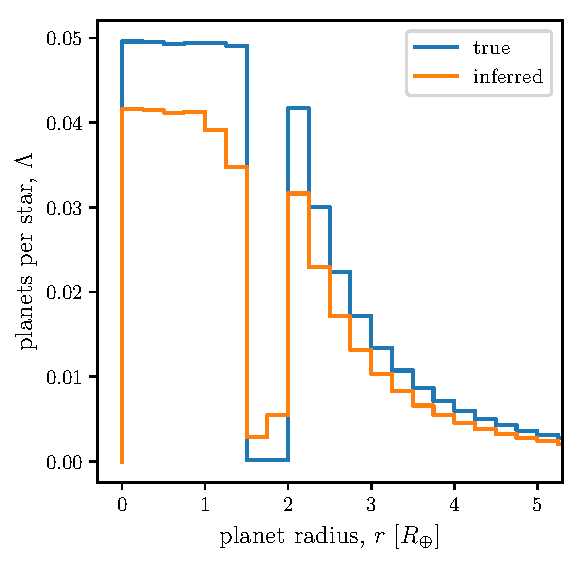
\includegraphics[width=.6\textwidth]{figures/rate_density_vs_radius_model_4_xcut.pdf}
    \caption{
        Inferred planet occurrence rates as a function of planet radius in 
        a model with a radius gap (Eq.~\ref{eq:model4_radius_distribution}).
        Similar to Model \#3, this model has fixed primaries and single stars, 
        but varying secondaries.
    }
    \label{fig:model_4}
\end{figure}
Using improved stellar parameters measured by the California-{\it Kepler} 
survey,~\citet{fulton_california-_2017} recently reported a ``gap'' in 
the radius-period 
plane~\citep{petigura_california-kepler_2017,johnson_california-kepler_2017}.
The existence of the gap has been independently corroborated from a sample of 
KOIs with asteroseismically-determined stellar 
parameters~\citep{van_eylen_asteroseismic_2017}.
Precise measurement of the gap's features, in particular its width, 
depth, and shape, will require more accurate occurrence rates.
To illustrate binarity's role in the issue, we make identical assumptions as 
in Model \#3, but instead assume an intrinsic radius distribution
\begin{align}
p_r(r)
&\propto
\left.
\begin{cases}
r^\delta & \text{for } r\geq 2r_\oplus, \\
0 & \text{for } 1.5r_\oplus < r < 2r_\oplus, \\
{\rm constant} & \text{for } r\leq1.5r_\oplus.
\end{cases}
\right.
\label{eq:model4_radius_distribution}
\end{align}
The resulting true and inferred rates are shown in Fig.~\ref{fig:model_4}.
If left uncorrected, binarity makes the gap appear more shallow, and flattens 
the step-function edges.
At present though, binarity seems less important than other effects that would 
``blur'' the gap in the planet radius dimension. 
In particular, the valley's period-dependence is almost certainly not flat
\citep{van_eylen_asteroseismic_2017,owen_evaporation_2017}.
This means that any study assessing its width, depth, etc. only in the planet 
radius dimension must first account for the blurring that comes from 
marginalizing over the periods.



\paragraph{Does a detected planet orbit the primary or secondary?}
\citet{ciardi_understanding_2015} studied the effects of stellar multiplicity 
on the planet radii derived from transit surveys.
They modeled the problem for {\it Kepler}\ objects of interest by matching a 
population of binary and tertiary companions to KOI stars, 
under the assumption that the KIC-listed stars were the primaries.
They then computed planet radius correction factors assuming that {\it 
Kepler}-detected planets orbited the primary or companion stars
with equal probability (their Sec. 5).
Under these assumptions, they found that any given planet's radius is on 
average underestimated by a multiplicative factor of 1.5.

Our models show that assuming a detected planet has equal probability of 
orbiting the primary or secondary leads to an overestimate of
binarity's population-level effects.
A planet orbiting the secondary does lead to extreme corrections, but these 
cases are rare outliers, because the searchable volume for secondaries is so 
much smaller than that for primaries.
Phrased in terms of the completeness, in our Model \#3 only $\sim 6\%$ of 
selected secondaries are searchable, compared to $\sim 60\%$ of selected 
primaries.
This means that when high-resolution imaging discovers a binary companion in 
a system that hosts a detected transiting planet, the planet is much
more likely to orbit the primary.
This statement is independent of the fact that planets are often confirmed to 
orbit the primary by inferring the stellar density from the transit duration.


\paragraph{On the utility for future occurrence rate measurements}
{\it TESS}\ is expected to discover over $10^4$ giant 
planets~\citep{sullivan_transiting_2015}.
Though they will be difficult to distinguish from false positives, one 
possible use of this overwhelmingly large sample will to measure an
occurrence rate of short-period giant planets.
Our work indicates that if this measurement is to be more accurate than $\sim 
30\%$, binarity cannot be neglected.


\paragraph{Independent approaches for estimating binarity's effects}
T. Barclay et al.\! (in preparation) have performed the exercise of taking 
stars selected by the {\it Kepler}\ team, pairing them with a population of 
secondaries, injecting a realistic distribution of planet radii, 
and then comparing the inferred occurrence rates with the true ones.
In their model, they find that binarity leads to an inferred rate of 
Earth-sized planets $\approx 10\%$ less than the true rate.
In our Model \#3, if all $Z_i$'s are equal (a plausible assumption in 
the lack of evidence to the contrary), the underestimate is by a comparable 
16\%.